% CS615A Aspects of System Administration
% Author: Jan Schaumann <jschauma@netmeister.org>
% $Id: slides.tex,v 1.12 2006/02/27 02:53:29 jschauma Exp $
\special{! TeXDict begin /landplus90{true}store end }

\documentclass[xga]{xdvislides}
\usepackage[landscape]{geometry}
\usepackage{graphics}
\usepackage{graphicx}
\usepackage{colordvi}

\begin{document}
\setfontphv

%%% Headers and footers
\lhead{\slidetitle}                               % default:\lhead{\slidetitle}
\chead{CS615 - Aspects of System Administration}% default:\chead{\relax}
\rhead{Slide \thepage}                       % default:\rhead{\sectiontitle}
\lfoot{\Gray{Automating Administrative Tasks}}% default:\lfoot{\slideauthor}
\cfoot{\relax}                               % default:\cfoot{\relax}
\rfoot{\Gray{\today}}

\vspace*{\fill}
\begin{center}
	\Hugesize
		CS615 - Aspects of System Administration\\ [1em]
		Automating Administrative Tasks / Shell Scripting\\ [1em]

	\hspace*{5mm}\blueline\\ [1em]
	\Normalsize
		Department of Computer Science\\
		Stevens Institute of Technology\\
		Jan Schaumann\\
		\verb+jschauma@stevens.edu+\\
		\verb+http://www.cs.stevens.edu/~jschauma/615/+
\end{center}
\vspace*{\fill}

\subsection{Midterm Survey}
\vspace*{\fill}
\begin{center}
\begin{verbatim}
https://www.cs.stevens.edu/~jschauma/cgi-bin/midterm.cgi
\end{verbatim}
\end{center}
\vspace*{\fill}

\subsection{Repeating Jobs}
Humans are terrible at remembering to do something repeatedly and
regularly.  We should let computers do that. \\

\vspace{.5in}

Enter \verb+cron(8)+ / \verb+crontab(5)+.

\subsection{Repeating Jobs}
Example: \\
\vspace{.5in}

\begin{verbatim}
30 2 * * 7 find /tmp -type f -mtime +7 -atime +7 -exec rm -f '{}' ';'
\end{verbatim}

\subsection{Time is relative}
Sometimes an hour doesn't exist. \\

\vspace{.5in}
Sometimes an hour repeats. \\

\vspace{.5in}
What happens to your \verb+crontab+?
\begin{verbatim}
30 2 * * 7 find /tmp -type f -mtime +7 -atime +7 -exec rm -f '{}' ';'
\end{verbatim}

\subsection{Time is relative}
Sometimes an hour doesn't exist. \\

\vspace{.5in}
Sometimes an hour repeats. \\

\vspace{.5in}
All sorts of other things you thought were true are not: \\
\verb+http://infiniteundo.com/post/25326999628/falsehoods-programmers-believe-about-time+

\subsection{Current Events}
CVE-2015-0204: FREAK attack \\

\verb+https://freakattack.com/+ \\

\verb+http://is.gd/5UfDHE+ \\

\verb+http://is.gd/QjuRWX+

\subsection{Regular Expressions 101}
A {\em regular expression} is a pattern that describes a set of strings. \\

\begin{itemize}
	\item patterns can be
		\begin{itemize}
			\item single characters (\verb+a+)
			\item a bracket expression, such as
				\begin{itemize}
					\item a set of characters -- \verb+[aK2l,]+
					\item a range expression -- \verb+[a-z]+
					\item a negated bracket expression -- \verb+[^0-9]+
				\end{itemize}
			\item a character with a special meaning, such as
				\begin{itemize}
					\item \verb+.+ -- any single character
					\item \verb+^+ -- beginning of line
					\item \verb+$+ -- end of line
				\end{itemize}
			\item a combination of patterns
		\end{itemize}
\end{itemize}

\subsection{Regular Expressions}
\begin{itemize}
	\item patterns can be followed by qualifiers and quantifiers
		\begin{itemize}
			\item \verb+?+ -- the pattern is optional and matched at most once
			\item \verb+*+ -- the pattern will be matched zero or more times
			\item \verb|+| -- the pattern will be matched one or more times
			\item \verb+{n}+ -- the pattern is matched exactly \verb+n+ times
			\item \verb+{n,}+ -- the pattern is matched \verb+n+ or more times
			\item \verb+{n,m}+ -- the pattern is matched at least \verb+n+,
				but no more than \verb+m+ times
		\end{itemize}
	\item patterns can be logically grouped together \verb+(1[a-z]2|a[0-9]z)+
	\item matched patterns can be remembered and referenced lateron
\end{itemize}
\addvspace{.5in}
NB: different tools/libraries implement regular expressions somewhat differently

\subsection{Regular Expressions}
Example exercises:
\begin{itemize}
	\item check if a string is a valid date
	\item check if a string is a valid IPv4 address
	\item check if a string is a valid IPv6 address
	\item extract all URLs from a document
	\item extract all proper words from a document
\end{itemize}

\subsection{Coding time!}
Page view statistics for Wikimedia projects \\
{\tt http://dumps.wikimedia.org/other/pagecounts-all-sites/} \\
{\tt https://wikitech.wikimedia.org/wiki/Analytics/Data/Pagecounts-all-sites} \\
\vspace{.5in}

On {\tt linux-lab.cs.stevens.edu}:
\begin{verbatim}
ls -l ~jschauma/public_html/615/pagecounts-20150201-000000
\end{verbatim}
\vspace{.5in}
Format: \\
\verb+    domain page_title count_views total_response_size+

\subsection{Coding time!}
How many unique objects were requested?

\subsection{Coding time!}
How many unique objects were requested?

\begin{verbatim}
FILE=~jschauma/public_html/615/pagecounts-20150201-000000
cat ${FILE} | wc -l
\end{verbatim}

\subsection{Coding time!}
How many unique objects were requested for {\tt en} only?

\subsection{Coding time!}
How many unique objects were requested for {\tt en} only?
\begin{verbatim}
grep -i "^en " ${FILE} | wc -l
grep -c -i "^en " ${FILE}
\end{verbatim}

\subsection{Coding time!}
Which is the most often requested object?

\subsection{Coding time!}
Which is the most often requested object?
\begin{verbatim}
grep -i "^en " ${FILE} | sort -k3 -n | tail -1
\end{verbatim}

\subsection{Coding time!}
How many requests per second were handled during this hour?

\subsection{Coding time!}
How many requests per second were handled during this hour?
\begin{verbatim}
awk '{ sum=sum+$(NF-1); }; END { print sum/60/60; }' <${FILE}
\end{verbatim}

\subsection{Coding time!}
How much data was transferred in total?

\subsection{Coding time!}
How much data was transferred in total?
\begin{verbatim}
echo $(( $(awk '{ sum=sum+$NF; }; END { print sum; }' <${FILE})/1024/1024/1024 ))
\end{verbatim}

\subsection{Coding time!}
Which was the largest object requested?

\subsection{Coding time!}
Which was the largest object requested?
\begin{verbatim}
awk '{ s=$NF/$(NF-1); if (s>l) { l=s; n=$0; }}; END { print n; }' <${FILE}
\end{verbatim}

\subsection{Coding time!}
What is the longest word found on the ten most frequently retrieved pages?

\subsection{Coding time!}
What is the longest word found on the ten most frequently retrieved
English Wikipedia pages?

\begin{verbatim}
for f in $(grep -i "^en " ${FILE}| sort -k3 -n | tail -10 |
        sed -e 's/en \(.*\) [0-9]* [0-9]*/\1/'); do
        links -dump http://en.wikipedia.org/wiki/${f}
done |
tr '[:punct:]' ' ' |
tr '[:space:]' '\n' |
tr '[:upper:]' '[:lower:]' |
egrep '^[a-z]+$' |
awk '{ print length() " " $0; }' |
sort |
uniq |
sort -n |
tail -1
\end{verbatim}

\subsection{User Interface}
\\
\vspace*{\fill}
\begin{center}
	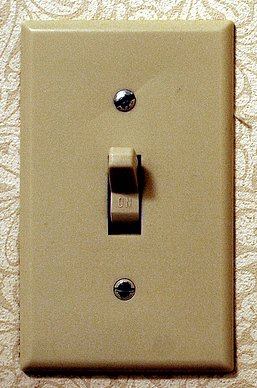
\includegraphics[scale=3]{pics/switch.eps}
\end{center}
\vspace*{\fill}


\subsection{Unix Philosophy}
\\
\Huge
\begin{center}
	Write programs that do one thing and do it well.\\
	\vspace{.5in}
	Write programs to work together. \\
	\vspace{.5in}
	Write programs to handle text streams, because that is a universal interface.
\end{center}
\Normalsize

\subsection{Know your languages / eco-system}
Some advice transcends language: \\

\begin{verbatim}
$ echo import this | python
\end{verbatim}

\subsection{The Zen of Python}
\Huge
\begin{center}
Beautiful is better than ugly.
\end{center}

\subsection{The Zen of Python}
\begin{center}
Explicit is better than implicit.
\end{center}

\subsection{The Zen of Python}
\begin{center}
    Simple is better than complex.
\vspace*{\fill}
	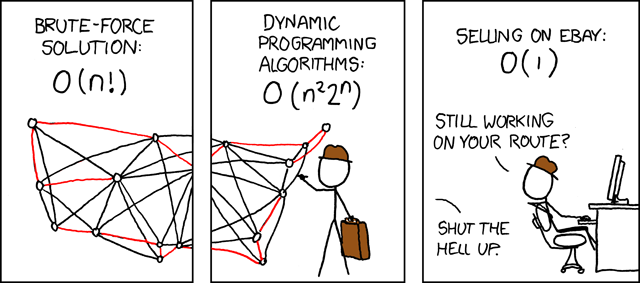
\includegraphics[scale=0.8]{pics/complexity.eps}
	\\
	\small \verb+http://xkcd.com/399/+
\end{center}
\vspace*{\fill}
\Huge

\subsection{The Zen of Python}
\begin{center}
    Complex is better than complicated.
\end{center}

\subsection{The Zen of Python}
\begin{center}
    Flat is better than nested. \\
    Sparse is better than dense. \\
\vspace{.5in}
    Readability counts.
\end{center}

\subsection{The Zen of Python}
\begin{center}
    Special cases aren't special enough to break the rules.
\end{center}

\subsection{The Zen of Python}
\begin{center}
    Special cases aren't special enough to break the rules. \\
\addvspace{.5in}
    Although practicality beats purity.
\end{center}

\subsection{The Zen of Python}
\\
\begin{center}
    Errors should never pass silently.
\end{center}

\subsection{The Zen of Python}
\\
\begin{center}
    Errors should never pass silently. \\
\addvspace{.2in}
	\small
	(That would be implicitly accepted failure.)
\end{center}
\Huge

\subsection{The Zen of Python}
\\
\begin{center}
    Errors should never pass silently. \\
\addvspace{.2in}
	\small
	(That would be implicitly accepted failure.) \\
\addvspace{.2in}
	(You know what would be better than something {\em implicit}?)
\end{center}

\subsection{The Zen of Python}
\\
\begin{center}
    Errors should never pass silently. \\
\addvspace{.2in}
	\small
	(That would be implicitly accepted failure.) \\
\addvspace{.2in}
	(You know what would be better than something {\em implicit}?) \\
\addvspace{.2in}
	(Why, of course, something {\em explicit}!)
\end{center}

\subsection{The Zen of Python}
\\
\begin{center}
    Errors should never pass silently. \\
\addvspace{.5in}
    Unless explicitly silenced.
\end{center}

\subsection{The Zen of Python}
\begin{center}
    In the face of ambiguity, refuse the temptation to guess.
\end{center}

\subsection{The Zen of Python}
\begin{center}
    There should be one -- and preferably only one -- obvious way to do it.
\end{center}

\subsection{The Zen of Python}
\begin{center}
    There should be one -- and preferably only one -- obvious way to do it.

\addvspace{.5in}

    Although that way may not be obvious at first unless you're Dutch. \\
\vspace*{\fill}
	
\includegraphics[scale=0.5]{pics/sign.eps}
\end{center}


\subsection{The Zen of Python}
\begin{center}
    Now is better than never.
\end{center}

\subsection{The Zen of Python}
\begin{center}
    Now is better than never.  \\

\addvspace{.5in}

    Although never is often better than *right* now.
\end{center}

\subsection{The Zen of Python}
\begin{center}
    If the implementation is hard to explain, it's a bad idea.
\end{center}

\subsection{The Zen of Python}
\begin{center}
    If the implementation is easy to explain, \\
	it {\em may} be a good idea.
\end{center}

\subsection{A simple interface, easy to explain.  Yet...}
\\
\vspace*{\fill}
\begin{center}
	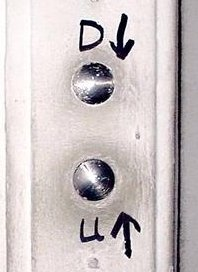
\includegraphics[scale=1.0]{pics/elevator_buttons-reverse.eps}
\end{center}
\vspace*{\fill}


\subsection{The Zen of Python}
\begin{center}
    Namespaces are one honking great idea -- let's do more of those!
\end{center}
\Normalsize

\subsection{Documentation}
\vspace*{\fill}
\begin{center}
	\includegraphics[scale=0.9]{pics/manual.eps}
	\hspace{.5in}
	\includegraphics[scale=0.9]{pics/manual2.eps}
	\\
	\vspace{.2in}
	\Huge
	{\bf WTFM}
	\Normalsize
\end{center}
\vspace*{\fill}

\subsection{Robustness Principle or Postel's Law}
\\
\Huge
\begin{center}
	Be conservative in what you do; be liberal in what you accept from others.
\end{center}
\Normalsize


\subsection{POLA}
Principle of Least Astonishment
\\
\vspace*{\fill}
\begin{center}
	
\includegraphics[scale=0.7]{pics/kinder-surprise.eps}
\end{center}
\vspace*{\fill}

\subsection{Know your Users}
Who do we automate things for?
\begin{itemize}
	\item ourselves
	\item our peers
	\item our "users"
	\item anybody else
\end{itemize}

\subsection{Avoid the Quick Fix}
\\
\Huge
\begin{center}
	There's nothing as permanent as a temporary solution.
\end{center}
\Normalsize

\subsection{Take a good look in the mirror!}
\\
\vspace*{\fill}
\begin{center}
	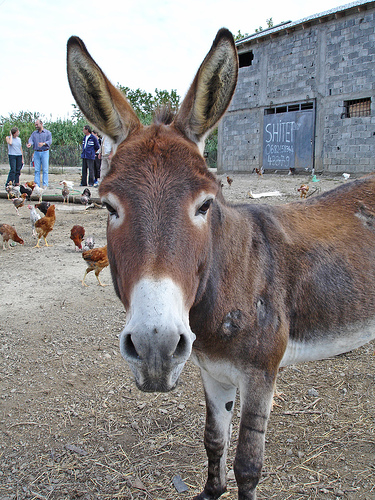
\includegraphics[scale=0.65]{pics/donkey.eps} \\
	\small
	Looks like {\em you} are the ass.
\end{center}
\vspace*{\fill}

\subsection{Learn to write a detailed bug report}
Pre-requisite:
\begin{itemize}
	\item RTFM
	\item Internet Search
	\item Know Your Community
\end{itemize}

\subsection{Learn to write a detailed bug report}
Pre-requisite: Do your homework. \\

Required:
\begin{itemize}
	\item Description Of Problem
	\item Steps To Reproduce
	\item Expected Results
	\item Actual Results
\end{itemize}

\subsection{Learn to write a detailed bug report}
Pre-requisite: Do your homework. \\

Required:
\begin{itemize}
	\item Description Of Problem
	\item Steps To Reproduce
	\item Expected Results
	\item Actual Results
\end{itemize}
\vspace{.125in}

Optional / recommended:
\begin{itemize}
	\item Screenshots / copy and paste terminal I/O
	\item Suggested Remediation
	\item Code Patch
\end{itemize}

\subsection{Avoid the Project That Was Never Finished}
\\
\Huge
\begin{center}
	Don't let the Perfect be the enemy of the Good.
\end{center}
\Normalsize

\subsection{Avoid Feature Creep}
\vspace*{\fill}
\begin{center}
	
\includegraphics[scale=1.0]{pics/feeping.eps} \\
	\small
	\verb+http://www.feepingcreatures.com+
\end{center}
\vspace*{\fill}

\subsection{Release Early, Release Often}
\\
\Huge
\begin{center}
	``More users find more bugs.'' \\
	\addvspace{.2in}
	\small F. Brooks, ``The Mythical Man Month''
\end{center}
\Normalsize

\subsection{Increase the Bus Factor}
\vspace*{\fill}
\begin{center}
	\includegraphics[scale=0.85]{pics/bert-ernie.eps} \\
	\small
	``Just friends.''
\end{center}
\vspace*{\fill}

\subsection{Fix Broken Windows}
\vspace*{\fill}
\begin{center}
	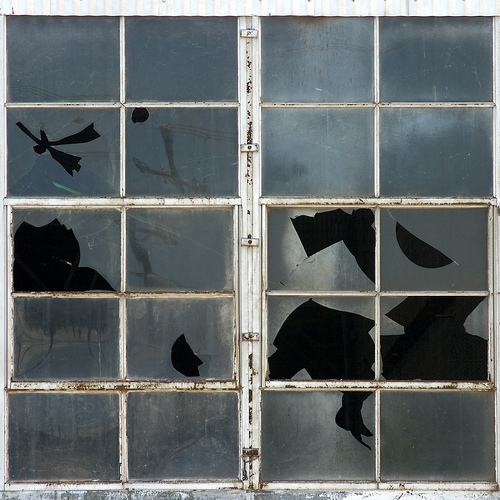
\includegraphics[scale=0.6]{pics/broken-windows.eps}
\end{center}
\vspace*{\fill}

\subsection{Program Maintenance}
\\
\Huge
\begin{center}
	``... is an entropy-increasing process, and even its most skillful
	execution only delays the subsidence of the system into unfixable
	obsolescence.'' \\
	\addvspace{.2in}
	\small F. Brooks, ``The Mythical Man Month''
\end{center}
\Normalsize

\subsection{Toss it!}
\vspace*{\fill}
\begin{center}
	
\includegraphics[scale=3]{pics/waste.eps}
\end{center}
\vspace*{\fill}

\newpage
\vspace*{\fill}
\begin{center}
    \Hugesize
        Hooray! \\ [1em]
    \hspace*{5mm}
    \blueline\\
    \hspace*{5mm}\\
        5 Minute Break
\end{center}
\vspace*{\fill}

\subsection{HW3}
\vspace*{\fill}
\begin{center}
\begin{verbatim}
https://www.cs.stevens.edu/~jschauma/615/s15-hw3.html
\end{verbatim}
\end{center}
\vspace*{\fill}


\subsection{Reading}
Shell:
\begin{itemize}
	\item \verb+http://www.tldp.org/HOWTO/Bash-Prog-Intro-HOWTO.html+
	\item \verb+http://www.tldp.org/LDP/abs/html/+
	\item \verb+http://sed.sourceforge.net/sed1line.txt+
	\item \verb+csh(1)+, \verb+ksh(1)+, \verb+sh(1)+
	\item {\em Frisch}: Chapter 3, 14
\end{itemize}
%Perl:
%\begin{itemize}
%	\item \verb+http://www.perl.com+
%	\item \verb+http://www.cpan.org+
%	\item \verb+perl(1)+, \verb+perldoc(1)+, \verb+perlfaq(1)+
%\end{itemize}
%Python:
%\begin{itemize}
%	\item \verb+http://www.python.org+
%	\item pydoc
%\end{itemize}

\end{document}
